\chapter{Sieci neuronowe}
\label{cha:sztuczne_sieci_neuronowe}

Rozdział ten zawiera informacje na temat historii rozwoju sieci neuronowych, ich architektury, zasady działania oraz algorytmów uczenia.

\section{Początki sztucznych sieci neuronowych}
Początki prac nad poznaniem procesów zachodzących w mózgu datuje się na rok 1943. W pracy McCulloch'a oraz Pitts'a przedstawiono matematyczny model neuronu, który zapoczątkował badania związane z tym tematem. W 1949 roku Donald Hebb odkrył, iż informacje przechowywane w sieci neuronowej są reprezentowane jako wartości wag pomiędzy poszczególnymi neuronami. Na podstawie tych informacji zaproponował on pierwszy algorytm uczenia sieci neuronowej, który został nazwany regułą Hebba. Już wtedy odkryto, iż bardzo dużą zaletą sieci jest równoległy sposób przetwarzania informacji oraz metodologia uczenia, która zastępuje tradycyjny proces programowania. 
%TODO dopisać więcej !!

\section{Sztuczne sieci neuronowe}
Sztuczne sieci neuronowe są często określane jako początki sztucznej inteligencji ze względu na ich sposób działania, który przypomina działanie ludzkiego mózgu. Korzystanie z sieci neuronowych wymaga przejścia przez dwa podstawowe etapy, pierwszy z nich określany jest jako uczenie sieci, a drugi testowanie, które jest używane do oceny poprawności działania sieci po jej wytrenowaniu. Istnieją różne algorytmy uczenia sieci neuronowej, najpopularniejszy z nich nazywany jest perceptron wielowarstwowy (ang. multilayer perceptron). Polega on na propagacji danych w przód, a następnie przy użyciu algorytmu wstecznej propagacji, modyfikacji odpowiednich wag neuronów. Sztuczne sieci neuronowe są uznawane jako skuteczna metoda do rozpoznawania wzorców. W ich skład wchodzą połączenia między neuronami jaki same neurony, które równolegle przetwarzają dane wejściowe. Podejście to zostało zainspirowane z biologicznego systemu nerwowego.

\section{Biologiczne neurony}

Ludzki mózg składa się z milionów neuronów, które są połączone między sobą przez prawie 10 miliardów synaps. Architektura ta pozwala na równoległe przetwarzanie informacji. Ogólny schemat biologicznego neuronu został przedstawiony na rysunku \ref{fig:bio_neuron}.

\begin{figure}[!htbp]
\centering
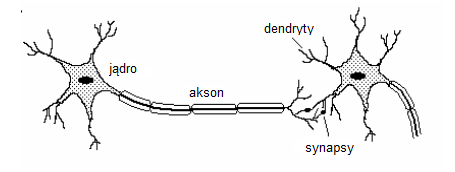
\includegraphics[width=1\linewidth]{./include/bio_neuron}
\caption{Biologiczny neuron.}
\label{fig:bio_neuron}
\end{figure}

Podstawową funkcję neuronu jest transportowanie przetworzonej informacji w postaci impulsu nerwowego, które są reprezentowane przez krótkotrwałą zmianę potencjału. Są one przewodzone od aksonu do synapsy która znajduje się na jego zakończeniach. 

\section{Sztuczny neuron}
Sposób działania sztucznego neuronu jest ściśle oparty na działaniu biologicznego neuronu. Posiada on wiele wejść oraz jedno wyjście. Dla lepsze zrozumienia funkcjonowania takiego neuronu wskażmy jego różnice w stosunku do biologicznego. %TODO zmienic cos
Współczesne komputery posiadają bardzo dużą moc obliczeniową skupiającej się w pojedynczych procesorach taktowanych wysoką częstotliwością. W odróżnieniu ludzki mózg posiada miliardy neuronów, które przetwarzają informacje wolniej niż współczesne procesory. Informacja przenoszona przez bodźce w ludzkim mózgu są reprezentowane przez logikę binarną o określonym progu aktywacji. W przypadku sztucznych neuronów funkcjonalność ta jest realizowane przez funkcje aktywacji, która na podstawie dobranego progu przypisuje wartość logiczną zbliżoną do "1" dla wartości powyżej oraz "0" dla pozostałych. W sztucznych sieciach neuronowych po wykonaniu obliczeń w konkretnym neuronie jego wartość wyjściowa przekazywana jest wzdłuż łańcucha sieci do kolejnych neuronów. 
W celu lepszego zobrazowania działania sztucznych neuronów często porównywane sa one do przekaźników. Synapsy występujące w ludzkim mózgu są odpowiednikami wag dla poszczególnych wejść neuronów.

\begin{figure}[!htbp]
\centering
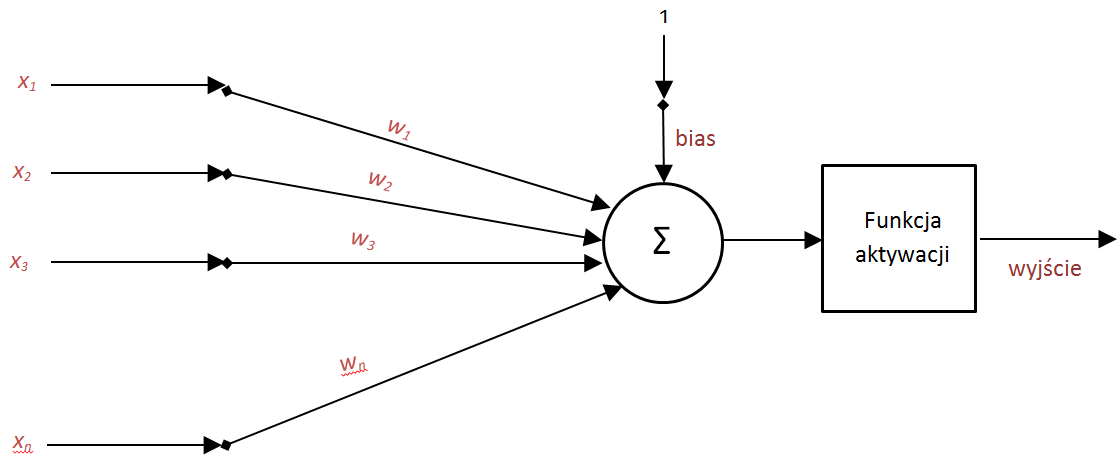
\includegraphics[width=1\linewidth]{./include/perceptron}
\caption{Sztuczny neuron.}
\label{fig:perceptron}
\end{figure}

Jak pokazano na rysunku \ref{fig:perceptron} wartości na każdym z wejść są przemnażane przez odpowiadające temu wejściu wagi. Jedno wejście posiada statyczną wartość 1, zabieg ten umożliwia sieci neuronowej lepiej przystosowywać się do wzorców. Neuron odpowiada za sumowanie wszystkich wartości. Następnie po obliczeniu sumy ilorazów wartości sygnałów wejściowych z poszczególnymi wagami, podawana jest ona na wejście funkcji aktywacji, której wyjście jest jednoznaczne z końcową wartością uzyskaną po przetworzeniu danego wektora wartości wejściowych. 

\section{Nauka sieci}

Nie jest możliwe aby w pełni za modelować pracę ludzkiego mózgu. Nie mniej jednak sztuczne sieci neuronowe pozwalają na rozwiązywanie wiele skomplikowanych zagadnień jak rozpoznawanie wszelkiego rodzaju wzorców oraz wiele innych. Bardzo ciekawą własnością sieci neuronowych jest to, iż nawet przy tej samej architekturze po ówczesnym przygotowaniu są w stanie one rozwiązywać całkowicie różne zagadnienia. Takie przystosowanie określane jest jako nauka sieci (ang. learning),proces ten można porównać do okresu rozwoju noworodka, który na podstawie zdobytych doświadczeń zdobywa nowe umiejętności.
Naukę dzieli się głównie na dwie podstawowe kategorie:
\begin{itemize}
	\item nauczanie z nauczycielem – (nadzorowane) (ang. supervised learning) –  podejście to wymaga nadzoru, w większości jest to zbiór oczekiwanych wartości odpowiedzi dla konkretnych wejść. Dokonuje się w nim próby przewidzenia wyników dla znanych danych wejściowych. Najbardziej znanym algorytmem w tej kategorii jest wsteczna propagacja błędów (ang. backpropagation). Polega ono na uczeniu sieci bazując na błędach. Początkowo wagi połączeń między neuronami są wybierane w sposób losowy, następnie na wejście sici podawany jest wektor wejść z znanymi poszczególnymi wartościami oraz znana jest również wartość oczekiwana dla wyjścia. Jest ona porównywana z aktualnym wyjściem sieci, a następnie na podstawie wielkości tego błędu wyliczana jest wartość korekcji poszczególnych wag każdego z połączeń, tak aby błąd ten został zminimalizowany. Największą wadą algorytmów tego typu jest znajomość dokładnej postaci wektora wyjściowego, która jest ciężka do spełnienia.
	\item nauczanie bez nauczyciela (nienadzorowane) (ang. unsupervised learning) - podejście to zyskało swoją popularność ze względu na brak konieczności znajomość oczekiwanego wektora danych wyjściowych podczas uczenia sieci. W tym przypadku wyjście sieci nie jest weryfikowane. Do najbardziej znanych algorytmów reprezentujących to podejście zaliczamy sieci Kohonena - samoograniczające się odwzorowania (ang. self-organizing map). Podczas podawania kolejnych danych uczących, to na sieci spoczywa odpowiedzialność za wytworzenie odpowiednich wzorców w zależności od danych wejściowych.
\end{itemize}
Istnieje możliwość wykorzystania obydwu metod uczenia odpowiednio ze sobą złączonych, które są stosowane oraz dają najlepsze rezultaty dla bardzo złożonych problemów.
 
\section{Funkcja aktywacji}
W sieciach neuronowych funkcja aktywacji odpowiedzialna jest za przekształcenie sumy powstałej przez dodanie iloczynów poszczególnych wag z odpowiadającymi im sygnałami wejściowymi. Wyróżnia się trzy główne typy takich funkcji: progowa, liniowa, sigmoidalna. 

\subsection{Progowa funkcja aktywacji}
Progowa funkcja aktywacji została przedstawiona przez McCullon'a oraz Pits'a w 1943 roku. Prosta funkcja tego typu może być określona wzorem:


$$ 
f(x) = \left\{ \begin{array}{ll}
+1 & \textrm{gdy $x>0$}\\
-1 & \textrm{gdy $x \le 0$}\\
\end{array} \right.
$$

Funkcja ogranicza się do przypisania zadanej wartości dla wejścia powyżej progu aktywacji. W pozostałych przypadkach neuron otrzymuje stan świadczący o braku jego aktywności. Na rysunku \ref{fig:step} przedstawiono przykładowy wykres funkcji progowej.

\begin{figure}[!htbp]
\centering
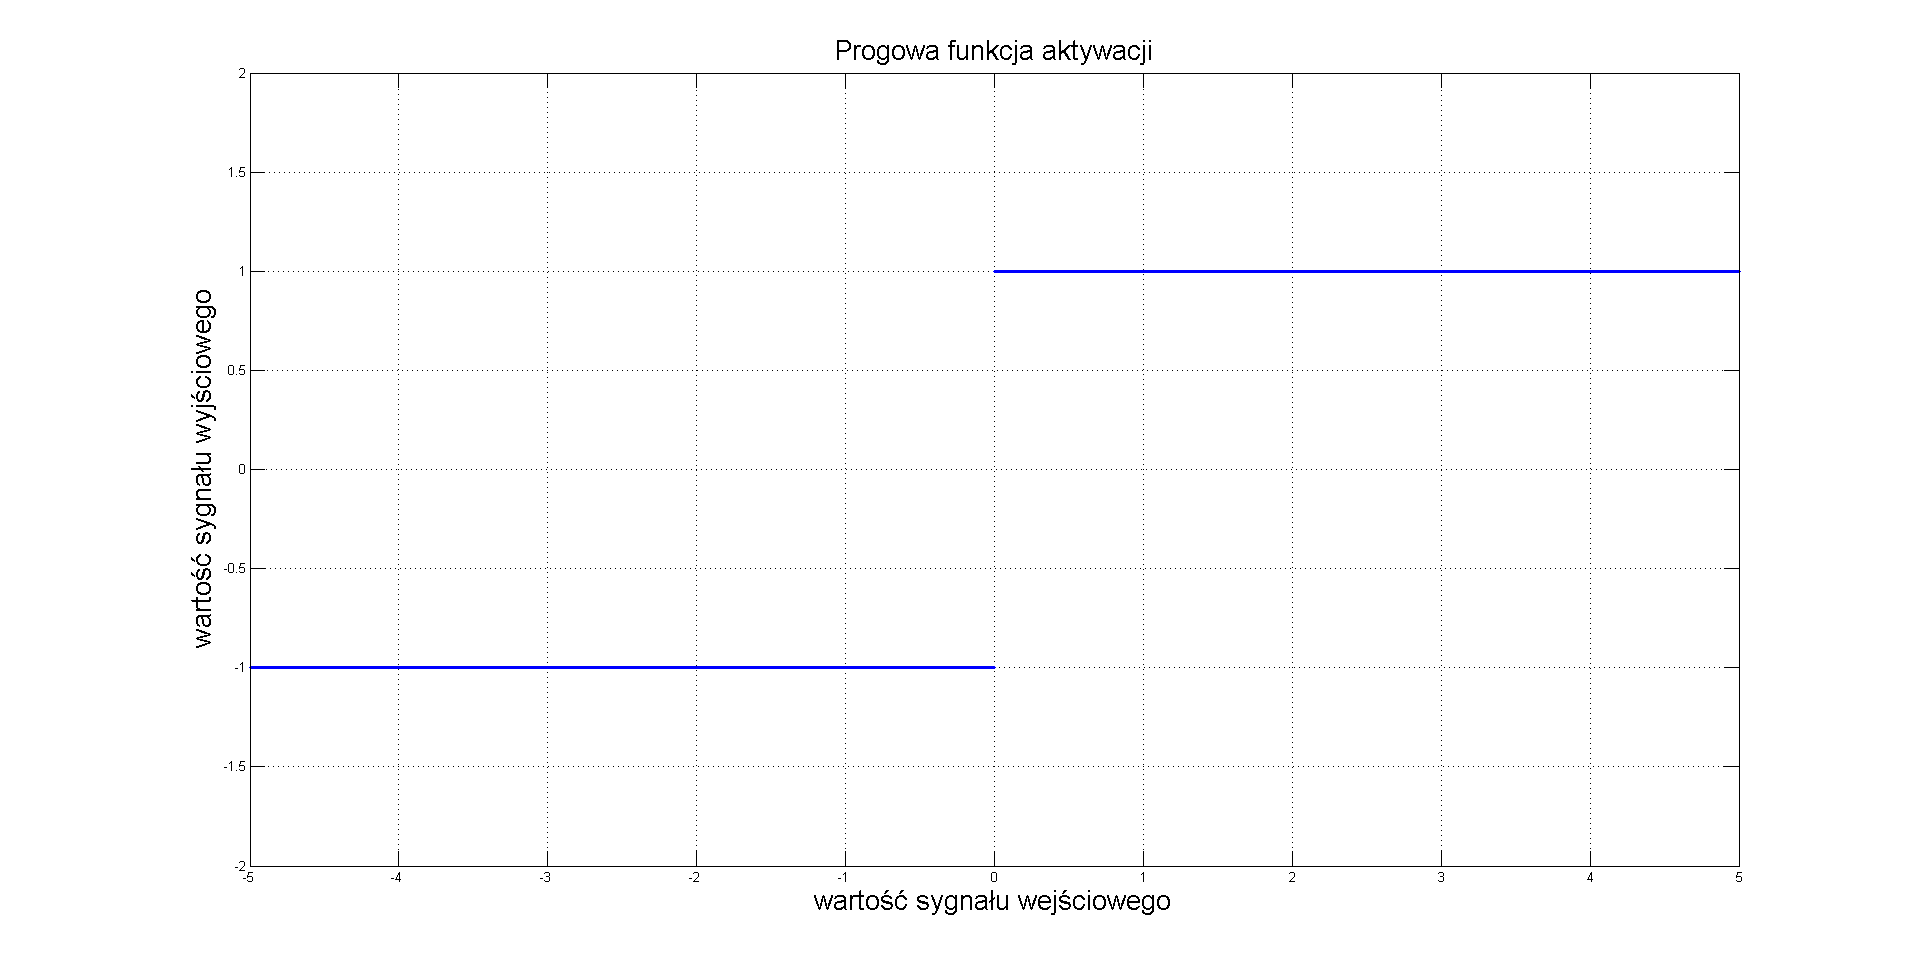
\includegraphics[width=1\linewidth]{./include/step}
\caption{Przykładowa funkcja progowa.}
\label{fig:step}
\end{figure}


\subsection{Liniowa funkcja aktywacji}
Funkcja liniowa odpowiada za liniowe przekazanie wartości wejściowej na wyjściową po przemnożeniu jej przez odpowiedni współczynnik. Dana jest ona wzorem:

$$ 
f(x) = a*x
$$

Na rysunku
\begin{figure}[!htbp]
\centering
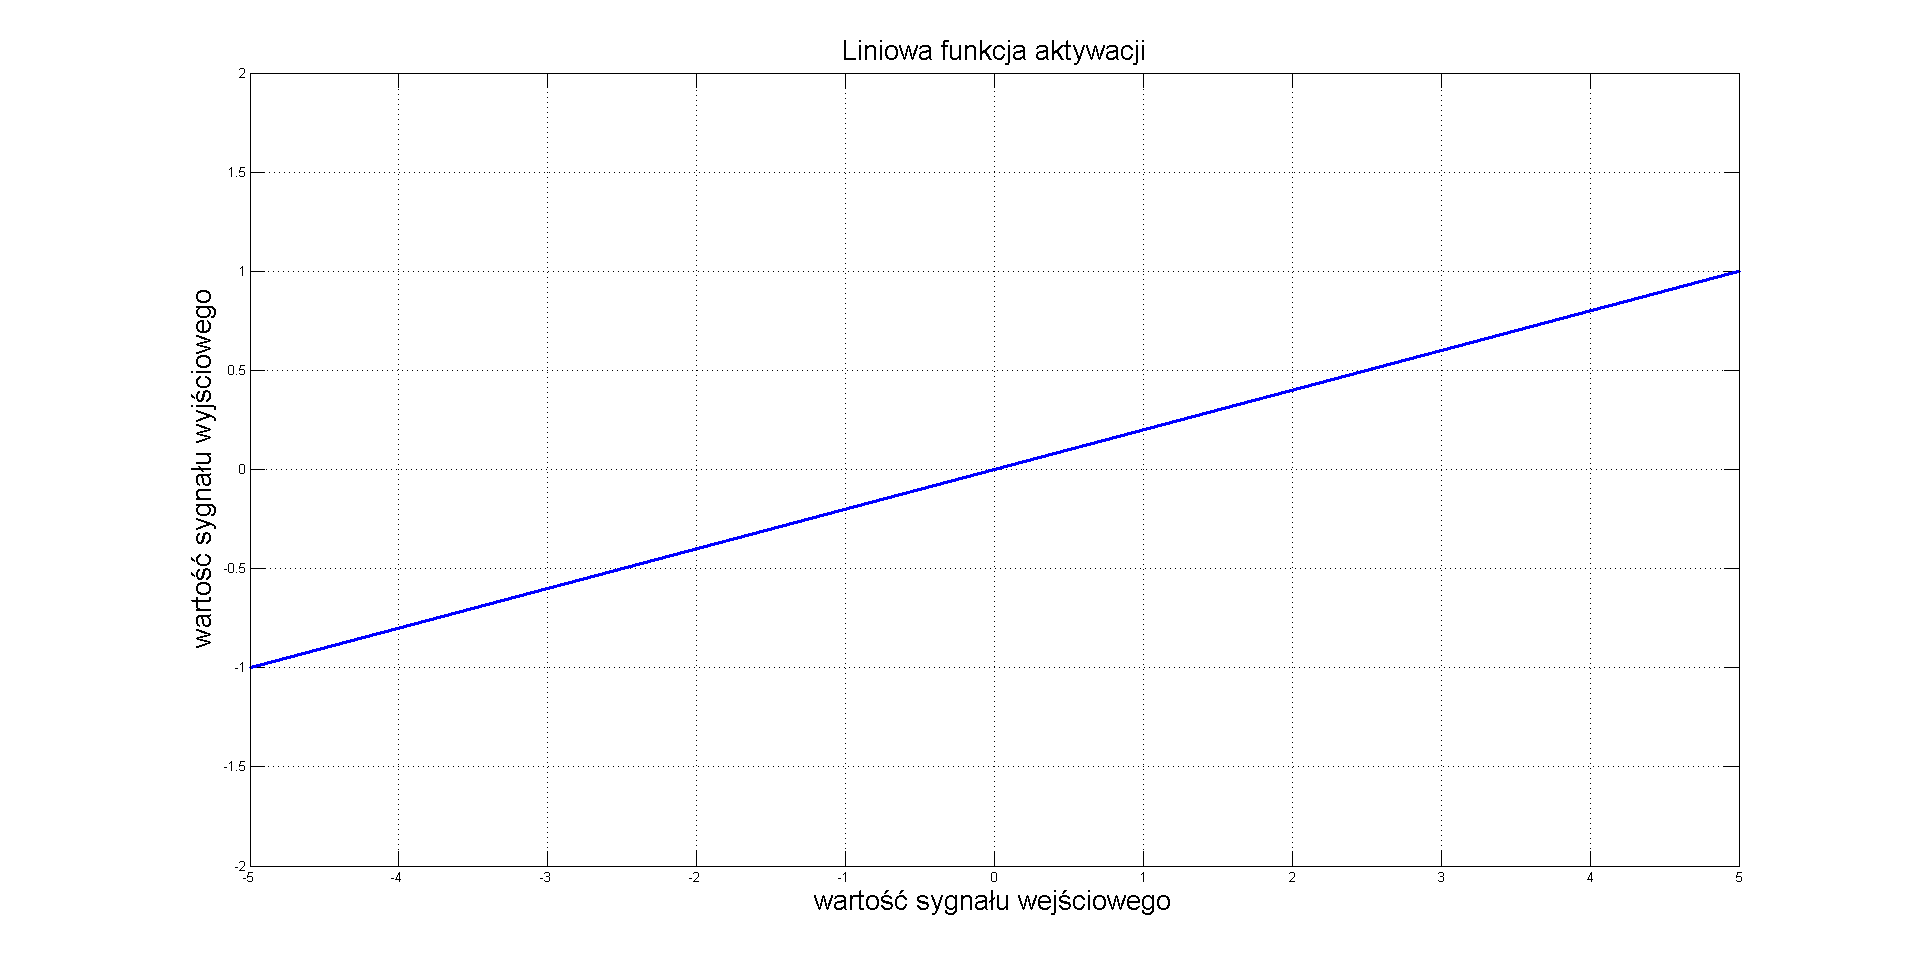
\includegraphics[width=1\linewidth]{./include/lin}
\caption{Przykładowa funkcja liniowa.}
\label{fig:lin}
\end{figure}

\subsection{Sigmoidalna funkcja aktywacji}
Funkcja sigmoidalna jest najczęściej używana w sztucznych sieciach neuronowych ze względu na jej różniczkowalność oraz zachowanie zgodne z głównym własnościami sieci neuronowych. Sigmoidalna funkcja unipolarna charakteryzuje się ona nieliniowym narastaniem w zakresie 0 do 1. Opisana jest wzorem:

$$ 
f(x) = \frac{1}{1 + e^{-x}}
$$

\begin{figure}[!htbp]
\centering
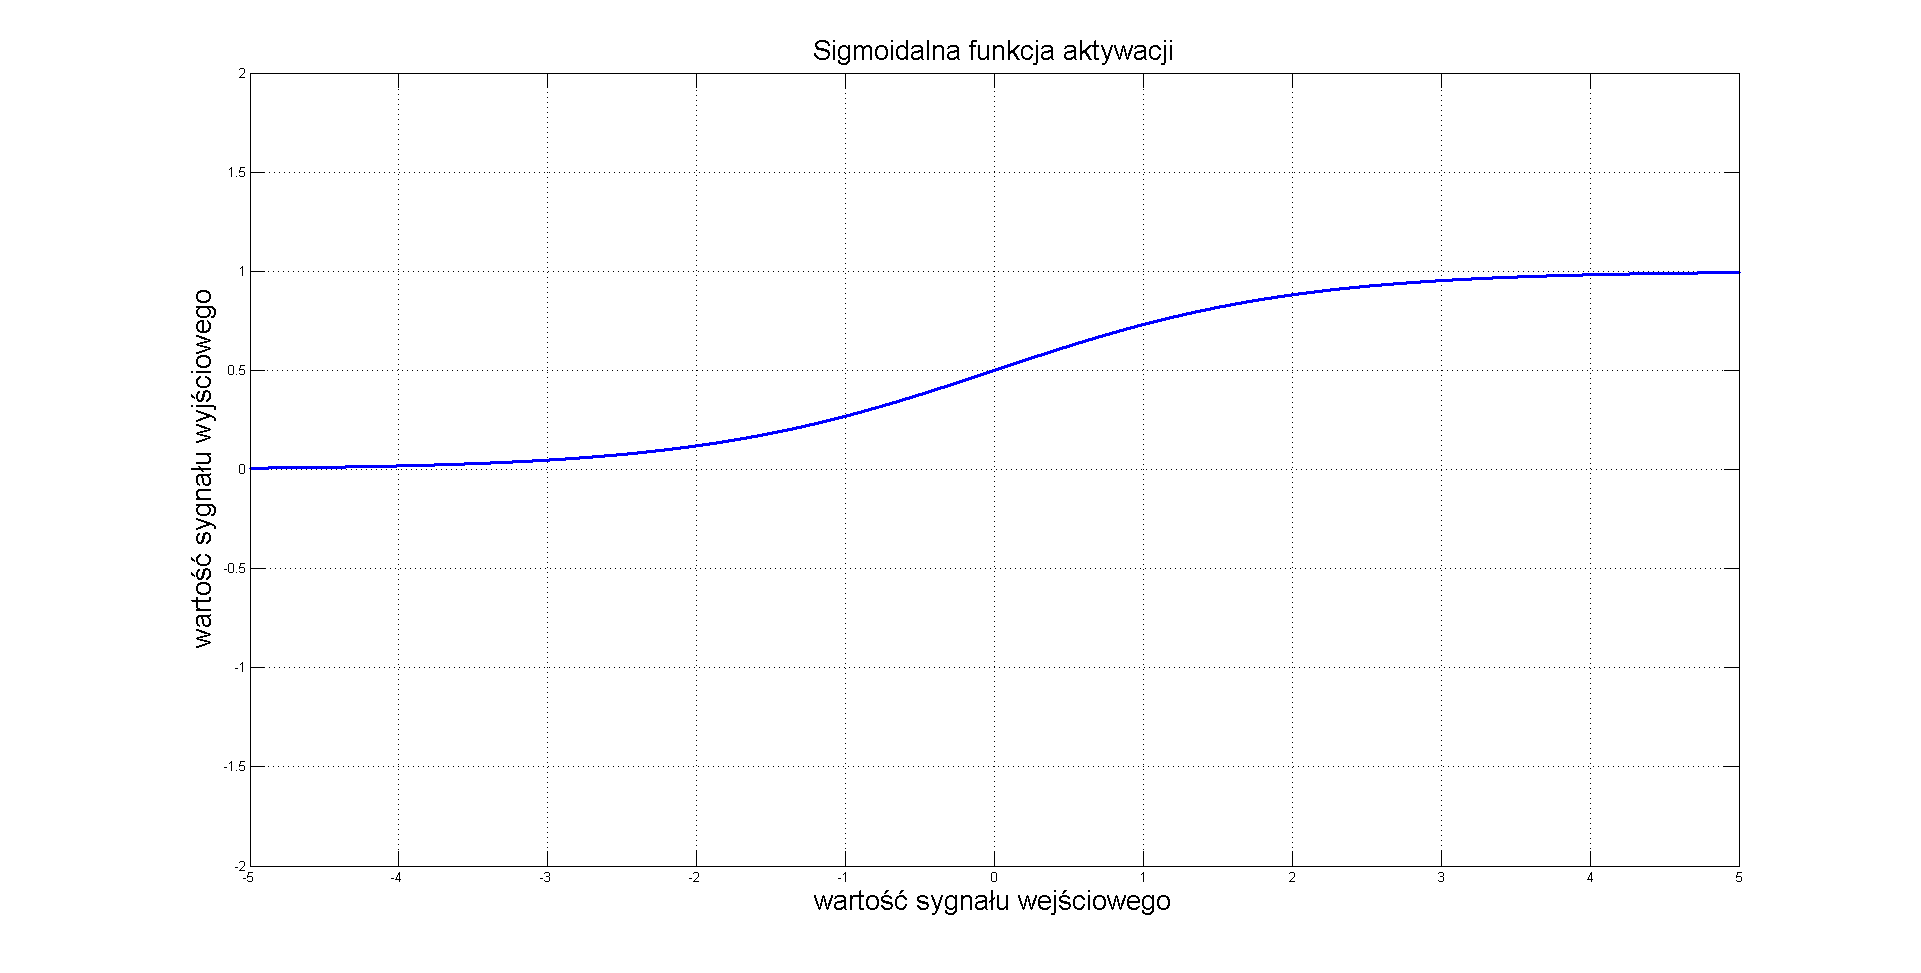
\includegraphics[width=1\linewidth]{./include/sig}
\caption{Wykres funkcji sigmoidalnej.}
\label{fig:sig}
\end{figure}

Bardzo często spotyka się również jej rozszerzoną wersję - bipolarną, która opisana jest wzorem tangensa hiperbolicznego:

$$ 
f(x) = \frac{1 - e^{-x}}{1 + e^{-x}}
$$

\begin{figure}[!htbp]
\centering
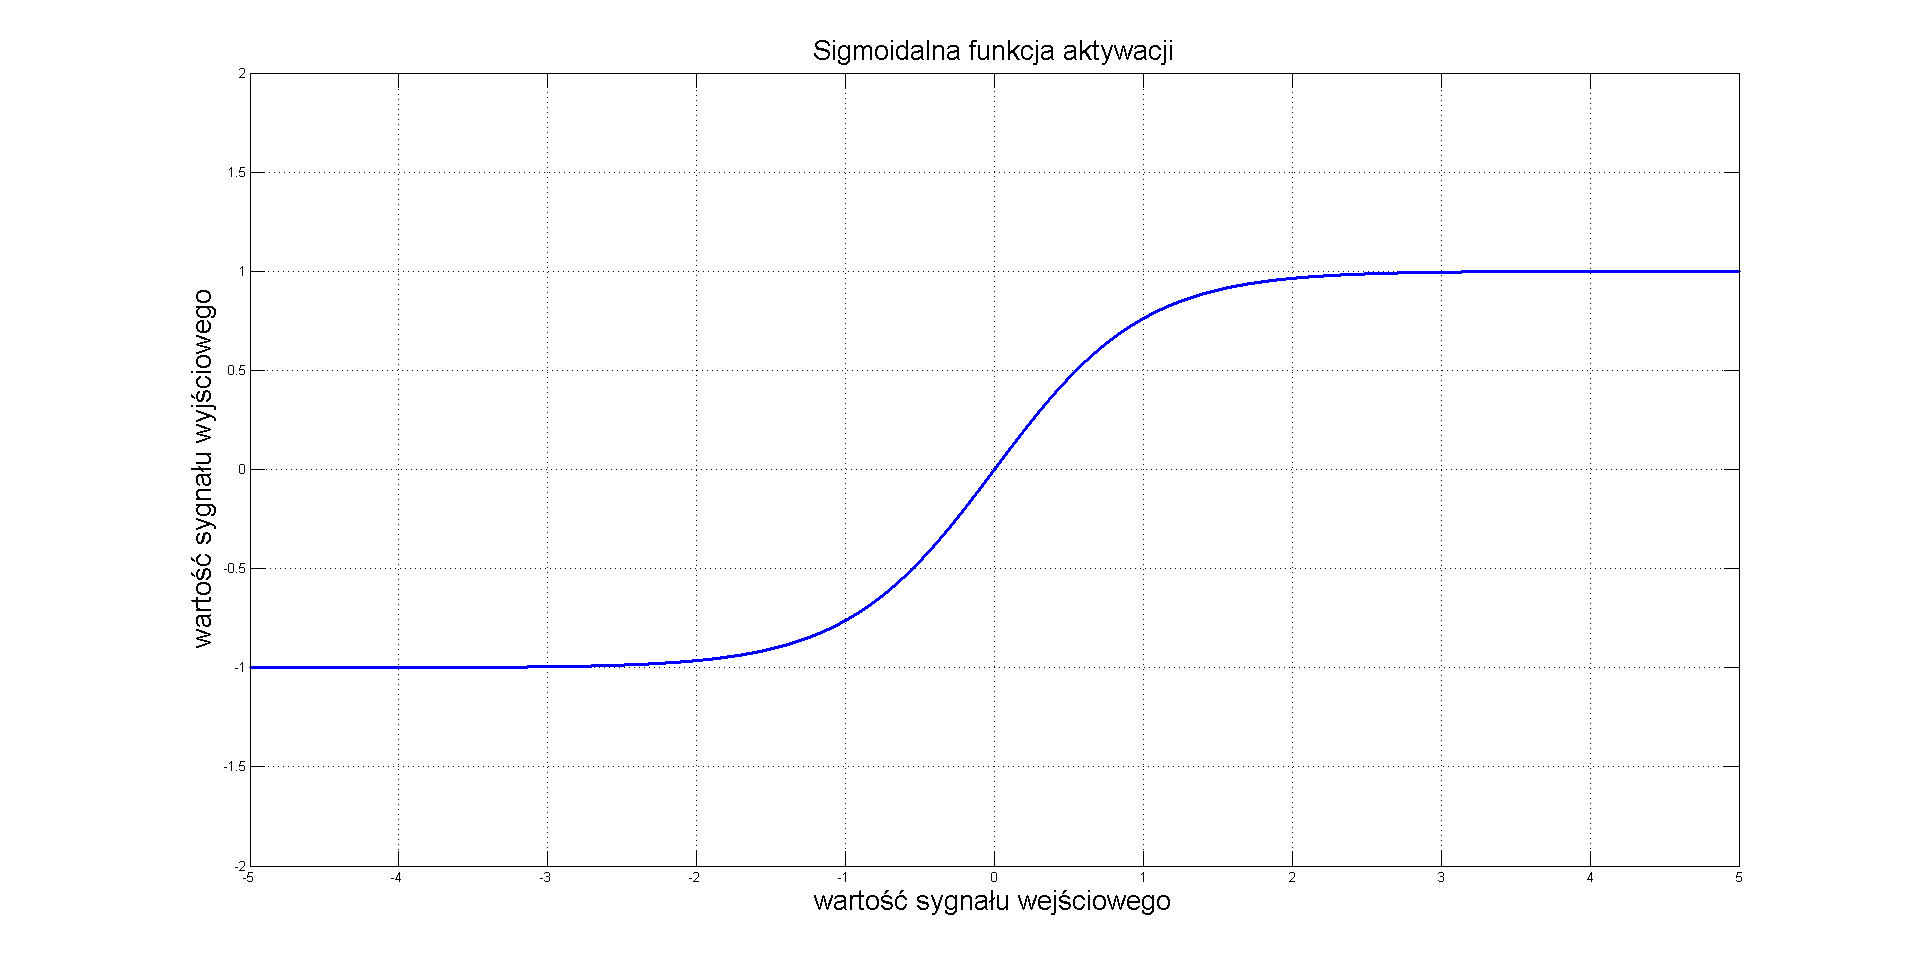
\includegraphics[width=1\linewidth]{./include/tanh}
\caption{Wykres funkcji tangensa hiperbolicznego.}
\label{fig:tanh}
\end{figure}

\section{Perceptron}
Perceptronem określa się sieć neuronową najprostszego typu, składającej się z neuronów McCullocha-Pittsa. Ich działania oparte jest na klasyfikacji sygnału wejściowego przez ustawieniu odpowiadający mu poziom wartości wyjściowej. 
Odbywa się to przez równoległe przemnożenie sygnałów wejściowych przez wagi połączeń na których się znajdują. Otrzymane ilorazy są sumowane,a następnie stanowią one wejście funkcji aktywacji której wyjście stanowi sygnał wyjściowy całego neuronu. Powyższe operacje zostały przedstawione na rysunku \ref{fig:flow}

\begin{figure}[!htbp]
\centering
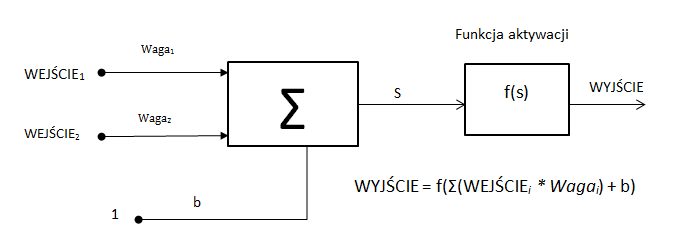
\includegraphics[width=1\linewidth]{./include/flow}
\caption{Schemat działania perceptronu.}
\label{fig:flow}
\end{figure}
 
 
Perceptrony posiadają zdolność klasyfikacji danych na charakterystyczne zbiory, które są liniowo separowalne. Własność ta pozwala tworzyć sieci w których aktywność poszczególnego neuronu oznacza przynależność do danego zbioru. Cecha ta uniemożliwia również wytrenowanie sieci jednowarstwowej, która rozwiązywała by problemy nieliniowe np. sieć wykonująca operację logiczną xor, która wymaga architektury posiadającej więcej niż jednej warstwy. 
Ze względu na tą własność pojedyncza warstwa neuronów nie jest szczególnie użyteczna. Dopiero łączenie kilku warstw pozwala na rozwiązywanie złożonych problemów nieliniowych co zdecydowanie zwiększa możliwości sieci neuronowej. 

\section{Backpropagation}

Do najbardziej popularnych algorytmów uczenia sieci zaliczany jest algorytm wstecznej propagacji błędu(ang. backpropagation). Głównym założeniem tego procesu jest korekcja wag wszystkich połączeń w sieci, które wpłynęły na zwiększenie błędu wynikającego z różnicy wartości oczekiwanej i rzeczywistej. W bardzo jasny oraz szczegółowy sposób algorytm został przedstawiony w książce %TODO tadeusiewicz.

Wyróżnia się dwie najważniejsze fazy, faza propagacji w przód, która podaje na wejście sieci wybrany wektor wejściowy ze zbioru danych uczących oraz odczytuje sygnał wyjściowy. Następną fazę określa się jako propagację wsteczną. Jej działania rozpoczyna się od ostatniej warstwy sieci do której podawana jest wartość błędu. Wykonywanie odwrotnych obliczeń wzdłuż sieci pozwala na wykrycie, które wagi wpłynęły na zwiększenie błędu a następnie korekcję ich wartości tak aby zminimalizować błąd.

%TODO RYSUNEK

Ze względu na istotne znaczenie tego procesu poniżej przedstawiono dokładny opis jego działania przedstawiony na pojedynczym neuronie.
Aby przystąpić do fazy nauki sieci należy odpowiednio przygotować zbiór danych uczących. Dane uczące dobierane są w ciąg o budowie opisanej wzorem \ref{eq:learning_data}.

\begin{equation}
U = <<X^{1}, z^{1}>, <X^{2}, z^{2}>,...,<X^{n}, z^{n}>>
\label{eq:learning_data}
\end{equation}

Jak łatwo zauważyć składa się on z par w postaci $<X^{j}, z^{j}>$, w których wyróżniamy wektor X z j-tym indeksem odpowiadający krokowi w procesie uczenia oraz przypisaną do niego informację o wartości oczekiwanej na wyjściu neuronu. Uwzględniając ówcześnie przedstawioną indeksację zbioru uczącego, regułę uczenia można opisać wzorem:

\begin{equation}
W^{j+1} = W^{j} + \eta^{j} \delta^{j} X^{j}
\label{eq:learning}
\end{equation}

We wzorze \ref{eq:learning} przyjęto:
\begin{equation}
\delta^{j} = z^{j} - y^{j}
\label{eq:delta}
\end{equation}
gdzie:
\begin{equation}
y^{j} = W^{j} * X^{j}
\label{eq:output}
\end{equation}

Reguła \ref{eq:learning} w pełni opisuje wszystkie konieczne do wykonania obliczenia. Warto jednak mieć na uwadze, iż wektor $W^{1}$ musi być określone. Bardzo często jest on inicjowany wartościami wybranymi losowo lub wartości te są przenoszone z poprzedniego procesu uczenia nawet jeśli jego zadaniem była realizacja zupełnie innej funkcji.
Bez względu na dobierane sposób inicjacji należy mieć na uwadze aby dobrane wartości były różne $\forall_{\eta, \nu} w^{1}_{\eta} \neq w^{1}_{\nu} $. Niespełnienie tego warunku może doprowadzić do braku postępów w początkowych procesie uczenia co wpływa na jego wydłużenie ewentualnie efekt końcowy. 

Bazując na powyższych oznaczenia można zapisać cel procesu uczenia. Celem tym jest doprowadzenie do zgodności wyjścia uczonego neurono $y^{j}$ z wartością oczekiwaną $z^{j}$, co jest jednoznaczne ze spełnieniem kryterium \ref{eq:crit}.

\begin{equation}
Q = \frac{1}{2} \sum_{j = 1}^{N} (z^{j} - y^{j})^{2}
\label{eq:crit}
\end{equation}

Dobrana funkcja $Q$ reprezentuje znaną metodę najmniejszych kwadratów.
Wzór ten można ogólnie przedstawić jako

\begin{equation}
Q = \sum_{j = 1}^{N} Q^{j}
\label{eq:common_crit}
\end{equation}

gdzie:

\begin{equation}
Q^{j} = \frac{1}{2}(z^{j} - y^{j})^{2}
\label{eq:condition_crit}
\end{equation}

Warto zauważyć, iż $Q = Q(W)$, zatem poszukiwanie minimum może odbywać się przy użyciu metody gradientowej, i-tą składową wektora $W$ można przedstawić jako:

\begin{equation}
w^{'}_i - w_{i} = \Delta w_{i} = - \eta \frac{\delta Q}{\delta w_{i}}
\label{eq:delta_member}
\end{equation}

W algorytmie backpropagation wyróżnia się poszczególne etapy:
\begin{enumerate}
	\item test
	\item test2
	\item test3
\end{enumerate}


Podczas efektywnej nauki korekty wag wraz z błędem na wyjściu sieci maleją z upływem czasu nauczania sieci. Zostaje on zakończony, gdy zostanie wykonana odpowiednia liczba iteracji na zbiorze uczącym lub błąd na wyjściu będzie poniżej zadanego progu. 






